\documentclass[11pt,a4paper]{article}
% \usepackage[MeX]{polski}
\usepackage[utf8]{inputenc}
\usepackage[T1]{fontenc}
\usepackage[polish]{babel}
\usepackage{graphicx}

\title{Projekt aplikacji}
\author{Łukasz A. Pelc}
\date{Styczeń 2021}

\begin{document}
    \thispagestyle{empty}
    \maketitle
    \newpage
    \section{Wygrane technologie}
    Technologie, które wybrałem do projektu:

    \begin{itemize}
        \item PostgreSQL -- mam duży doświadczenie z tą bazą danych,
        \item Django -- znam lepiej niż inne podobne frameworki i~ma wszystko w~sobie,
        \item Django REST Framework - jak Django to rozszerzenie do niego,
        \item Celery -- uruchamianie procesów,
        \item Redis -- wymaga Celery i~mam styczność z~tą bazą daych noSLQ,
        \item RabbitMQ -- wymagane przez Celery,
        \item Docker -- do uruchamiania wyżej wymienionych, aby nie instalować i~uruchamiać w~systemie,
        \item Docker-Compose -- aby łatwiej uruchamiać obrazy Dockera.
    \end{itemize}

    Kierowałem się ofertą jak i również własnym doświadczeniem czy zgłębieniem tematu. \\

    \section{Diagramy}
    \subsection{Diagram bazy danych ERD}

    \begin{figure}[!h]
        \begin{center}
            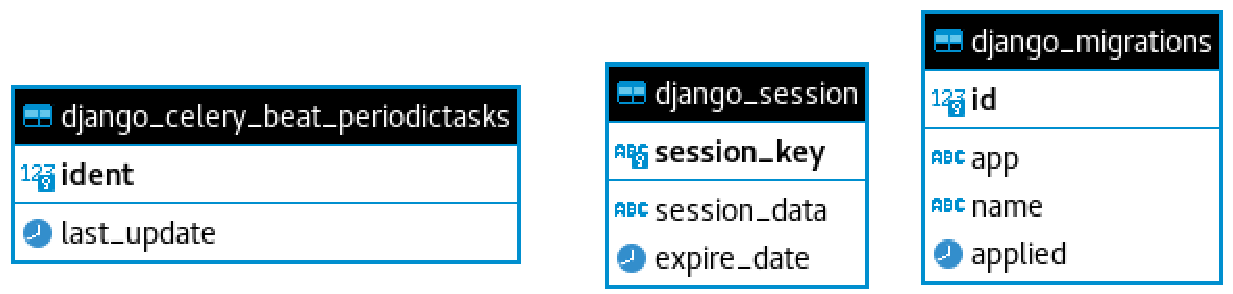
\includegraphics[width=\textwidth]{images/other_tables.pdf}
        \end{center}
        \caption{Tabele bez ralacji}
    \end{figure}
    \newpage
    \begin{figure}[!h]
        \begin{center}
            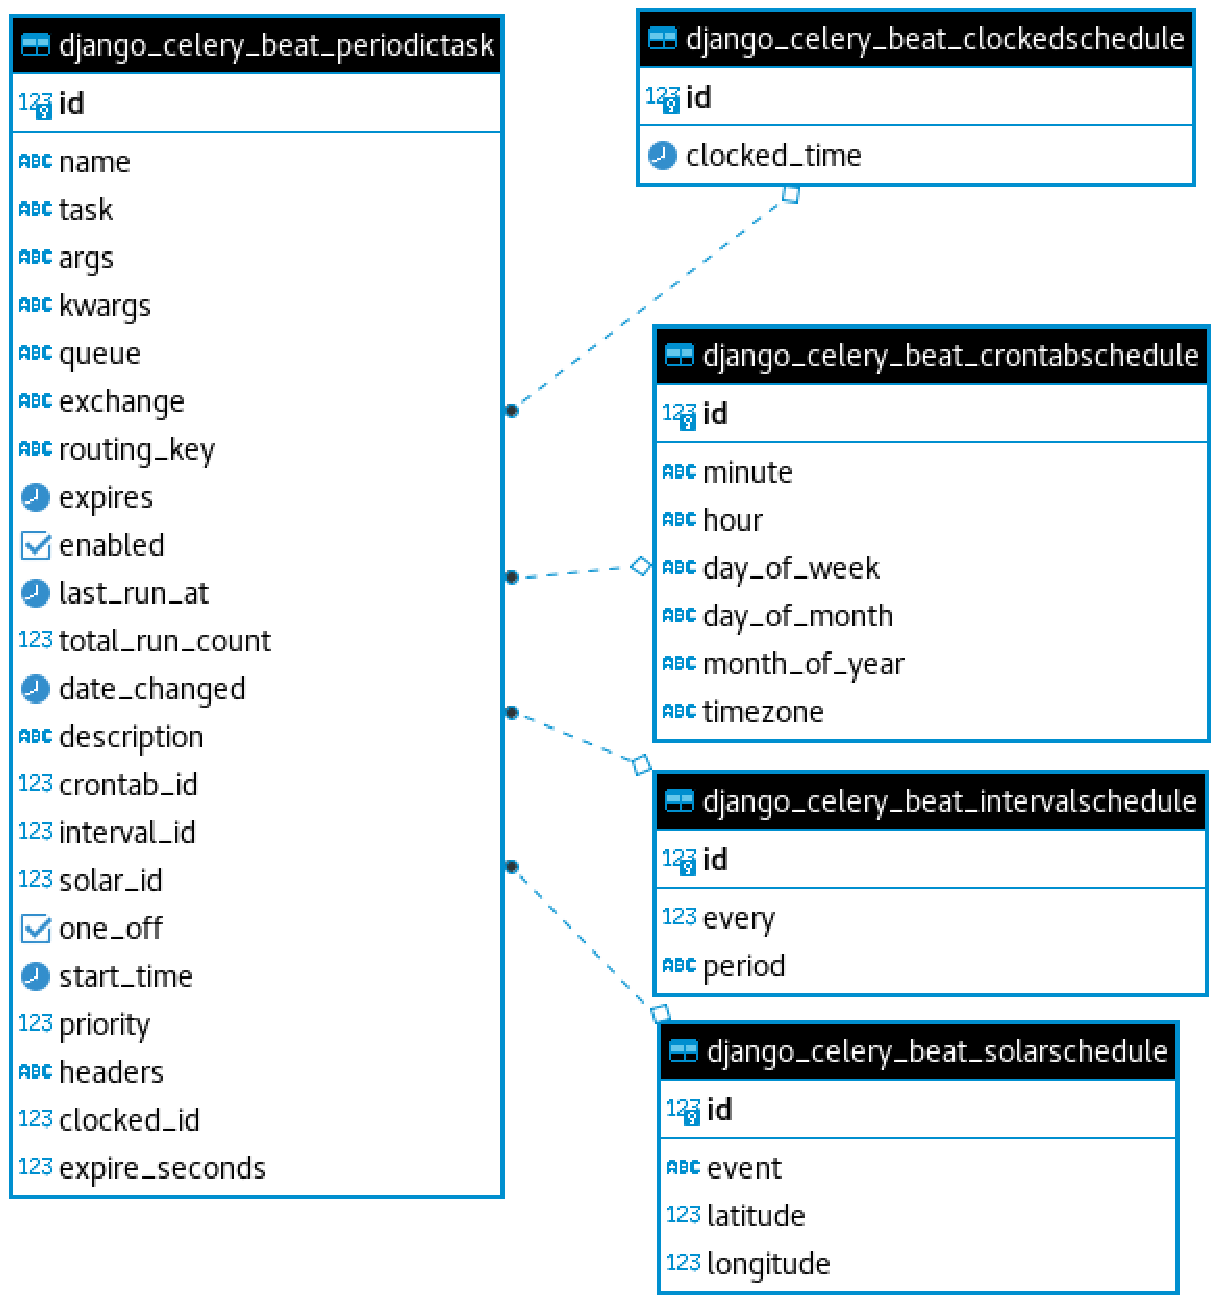
\includegraphics[width=\textwidth]{images/celery_tables.pdf}
        \end{center}
        \caption{Tabele Celery - pakiet django-celery-beat}
    \end{figure}

    \newpage
    \begin{figure}[!h]
        \begin{center}
            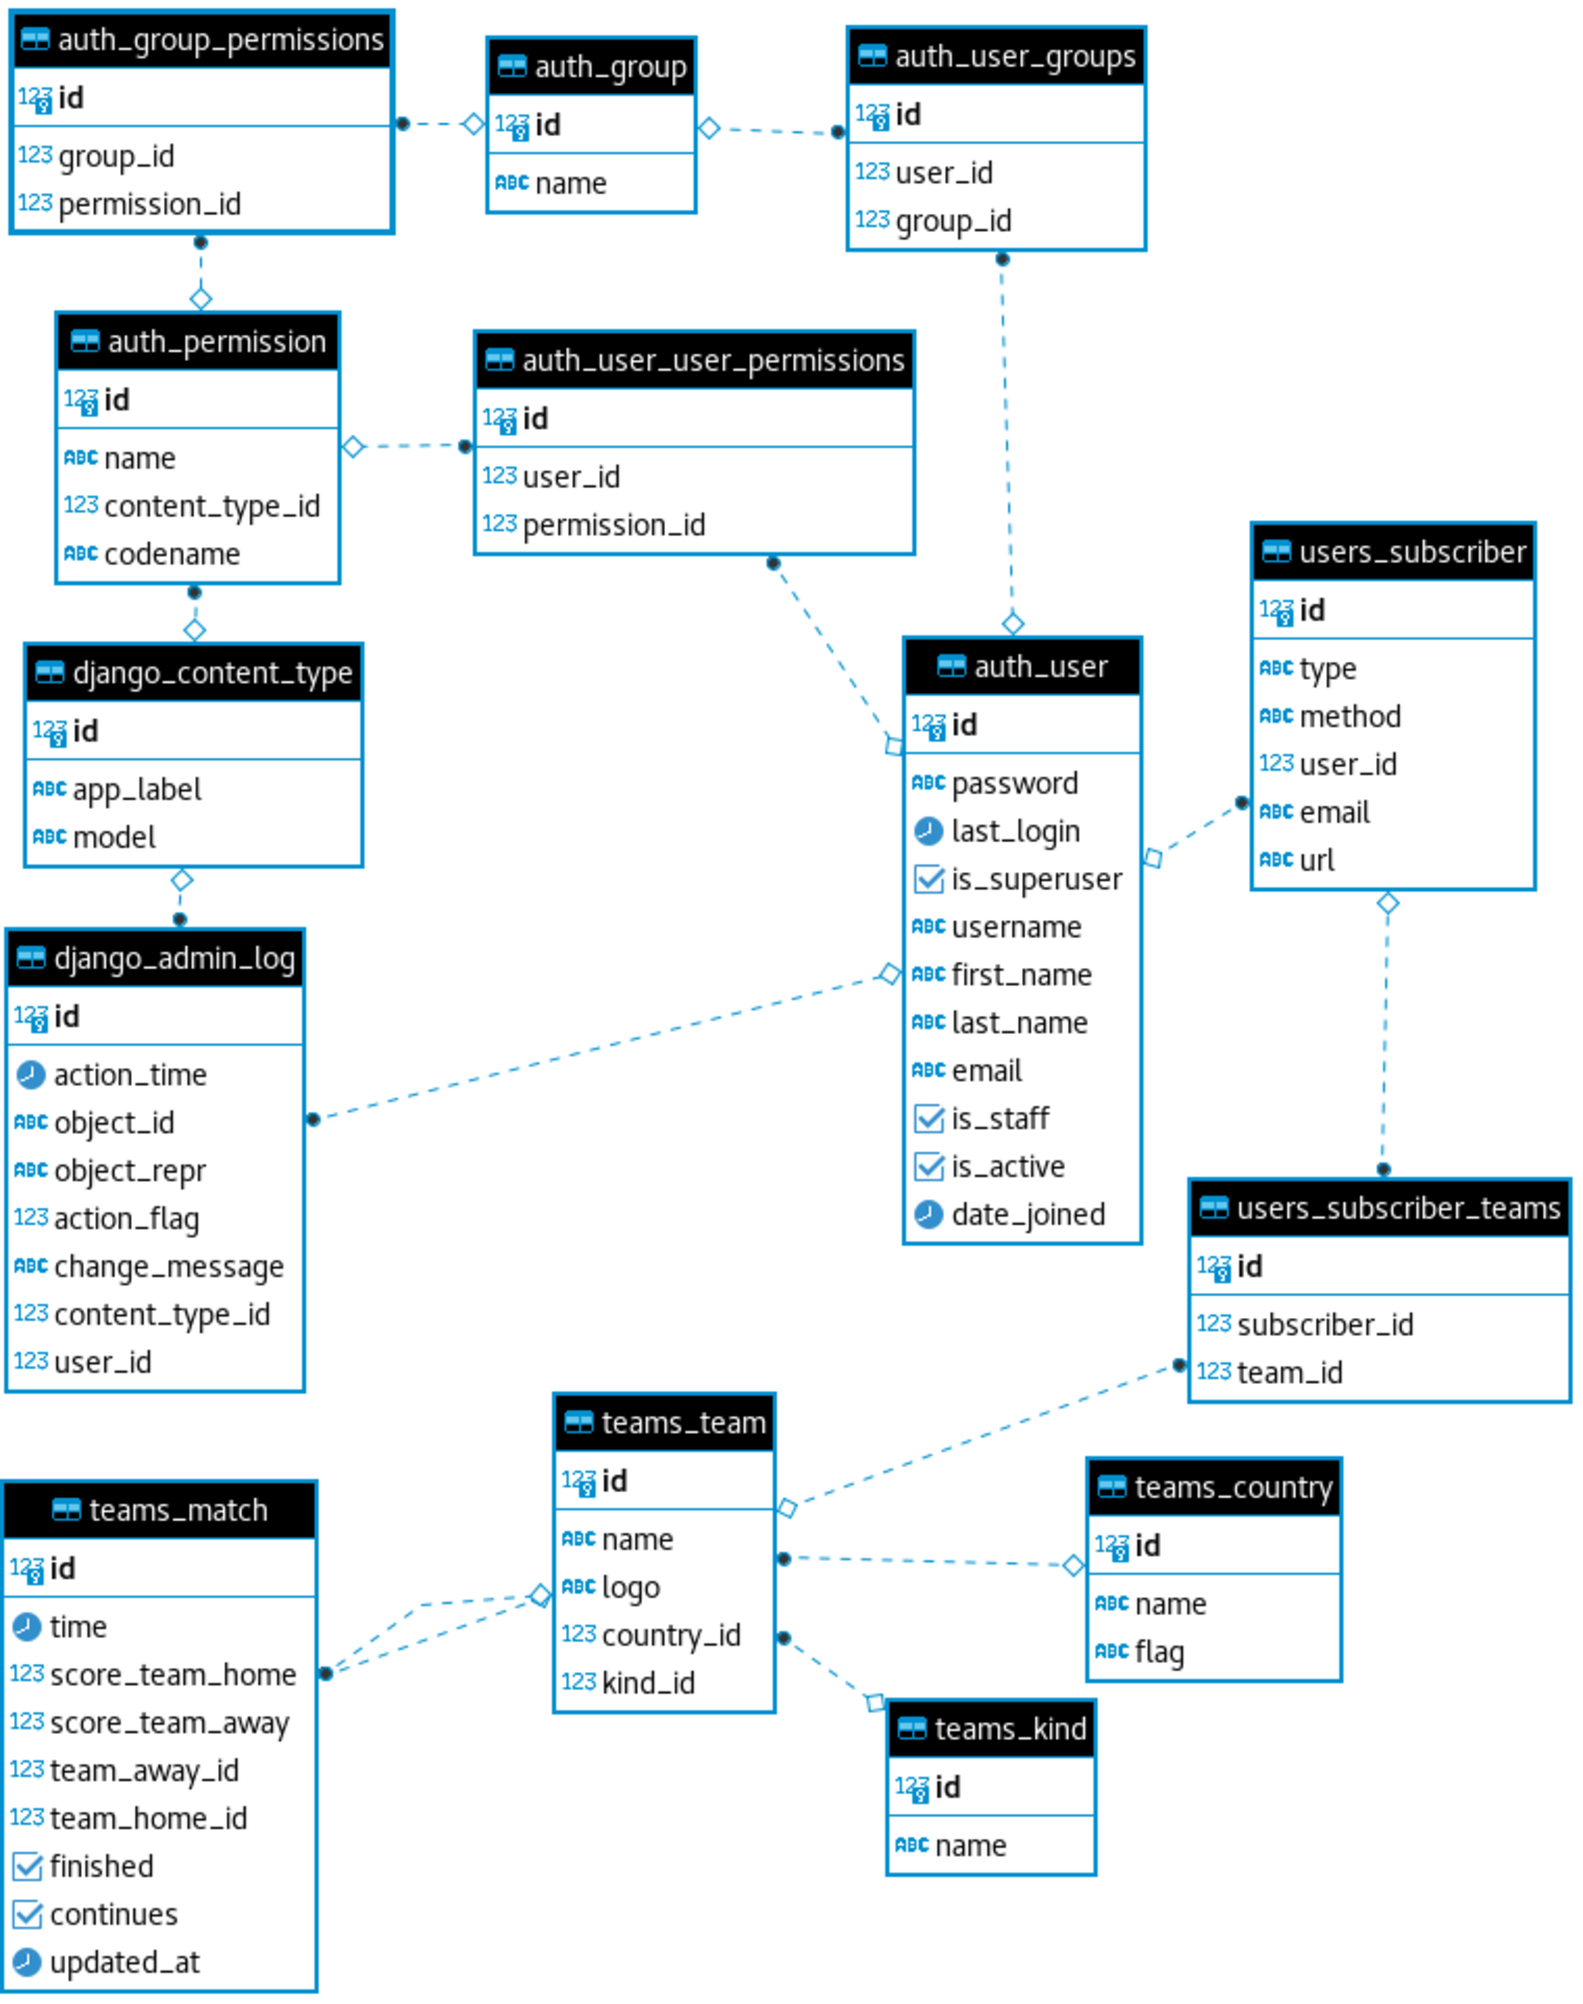
\includegraphics[width=\textwidth]{images/all_tables.pdf}
        \end{center}
        \caption{Tabele Django modułu auth i~tabele projektu}
    \end{figure}

    \newpage

    \subsection{Diagramy klas}

    \begin{figure}[!h]
        \begin{center}
            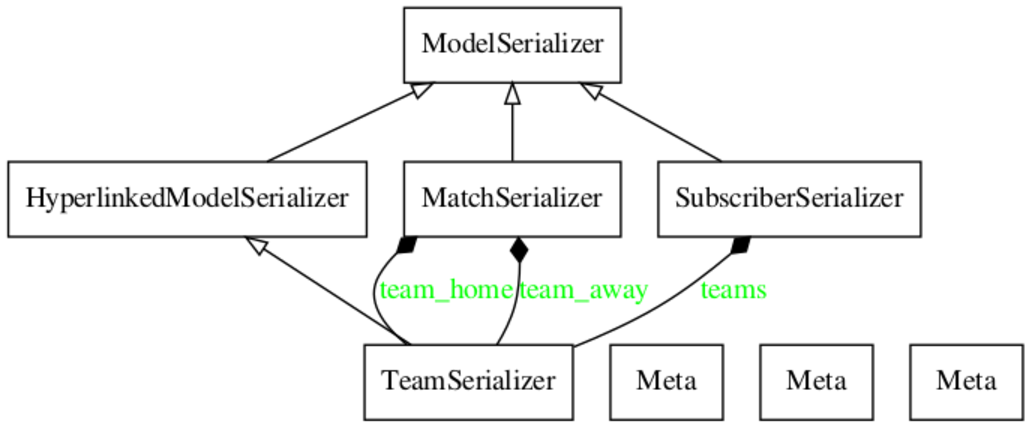
\includegraphics[width=\textwidth]{images/classes_api_serializers.pdf}
        \end{center}
        \caption{Klasy modułu api.serializers}
    \end{figure}

    \begin{figure}[!h]
        \begin{center}
            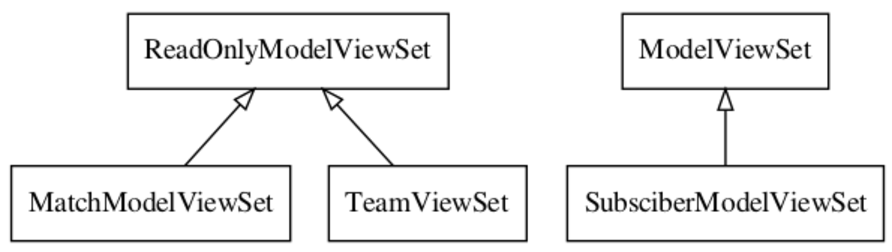
\includegraphics[width=\textwidth]{images/classes_api_views.pdf}
        \end{center}
        \caption{Klasy modułu api.views}
    \end{figure}

    \newpage

    \begin{figure}[!h]
        \begin{center}
            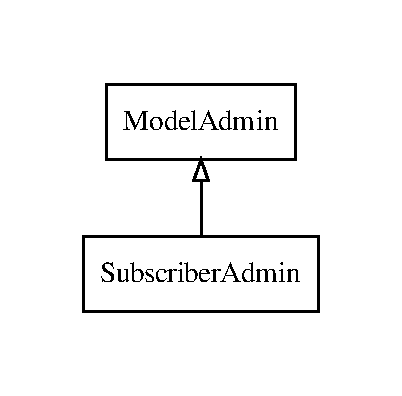
\includegraphics{images/classes_users_admin.pdf}
        \end{center}
        \caption{Klasy modułu users.admin}
    \end{figure}

    \begin{figure}[!h]
        \begin{center}
            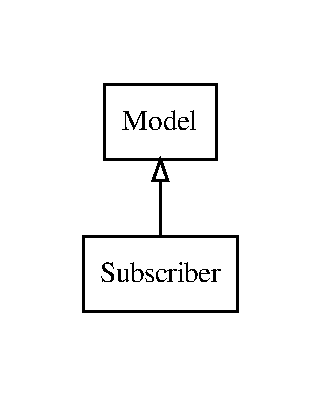
\includegraphics{images/classes_users_models.pdf}
        \end{center}
        \caption{Klasy modułu user.models}
    \end{figure}

    \begin{figure}[!h]
        \begin{center}
            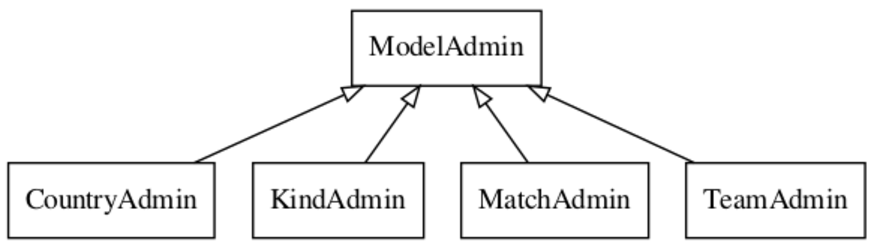
\includegraphics{images/classes_teams_admin.pdf}
        \end{center}
        \caption{Klasy modułu teams.admin}
    \end{figure}
    \begin{figure}[!h]
        \begin{center}
            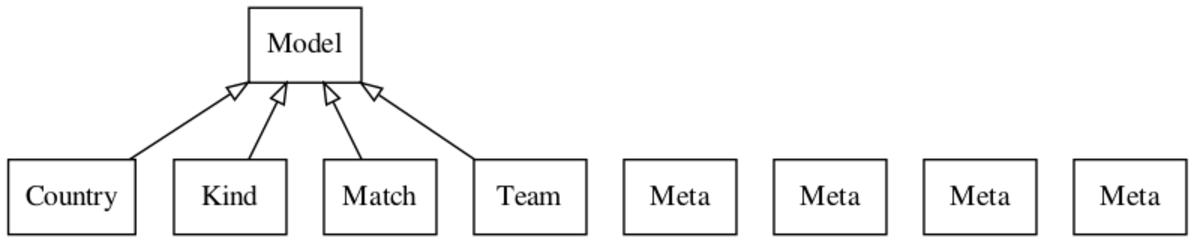
\includegraphics[width=\textwidth]{images/classes_teams_models.pdf}
        \end{center}
        \caption{Klasy modułu teams.models}
    \end{figure}


    \newpage

    \section{API}

    Wyświetlenie dostępnch drużyn: \\

    \begin{verbatim}
        GET http://127.0.0.1:8000/teams/
    \end{verbatim}

    Wyświetlenie subskrypcji: \\

    \begin{verbatim}
        GET http://127.0.0.1:8000/subscribe/",
    \end{verbatim}

    Zapisy subskrypcji: \\

    \begin{verbatim}
        POST http://127.0.0.1:8000/subscribe/

        DATA:
        {
            "type": "live",
            "method": "api",
            "teams": [2],
            "url": "http://host:10000/api/",
            "email":"",
            "token": ""
        }
    \end{verbatim}

    gdzie:

    \begin{itemize}
        \item type -- \verb+live+, \verb+day+ lub \verb+week+,
        \item method -- \verb+api+ lub \verb+api+,
        \item teams -- lista identyfikatorów (\verb+id+) drużyn,
        \item url -- URL zewnętrznego API,
        \item email -- e-mail adres, na który będzie wysyłany mail z~powiadomiwniem,
        \item token --  jeżeli jest potrzebny do połączenia z~zewętrznym API.
    \end{itemize}

    Wyświetlenie meczy lub spotkań: \\

    \begin{verbatim}
        GET http://127.0.0.1:8000/matches/
    \end{verbatim}

    Wyświetlenie tzech wygarzeń wydarzeń: \\

    \begin{verbatim}
        http://127.0.0.1:8000/matches/last_events/
    \end{verbatim}

    \section{Podsumowanie}

    Z~braku czasu nie zostały napisane testy i~tylko z~grusza aplikacja przetestowana tylko czy działa.
    Brak optymalizacji zapytań do bazy danych.\\

\end{document}
